\section{Implementation}

\subsection{General Idea}

The structure of the dataset, as well as, to be honest, recent labs of the
\textbf{Practical Machine Learning and Deep Learning} course inspire to use the
graph representation of the data.

We need to address the problem with corresponding tool. For instance, Graph
Neural Network~\cite{zhouGraphNeuralNetworks2020} seems to be pretty obvious
and good solution.

\subsection{Stack}

For such kind of task, especially the \textbf{GNN} we can use the corresponding
tools. For instance \textit{PyTorch}~\cite{PyTorch} and
\textit{PyG}~\cite{PyG}. Most of the testing was performed using \textit{Google
    Colab} capabilities, since I am \sout{proud} owner of the \textbf{AMD} graphics
card.

To properly address the properties of the data we may need the special
architecture. For example, \textit{Graph Convolutional Network}. Convolutional
layers may solve these questions. One of the possible solutions is
\textit{LightGCN}~\cite{heLightGCNSimplifyingPowering2020}. We may be
particularly interested in the structure of the convolutional layer
architecture and it is presented on the figure~\ref{fig:impl:lgc_arch}.

\begin{minipage}{\linewidth}
    \centering% 
    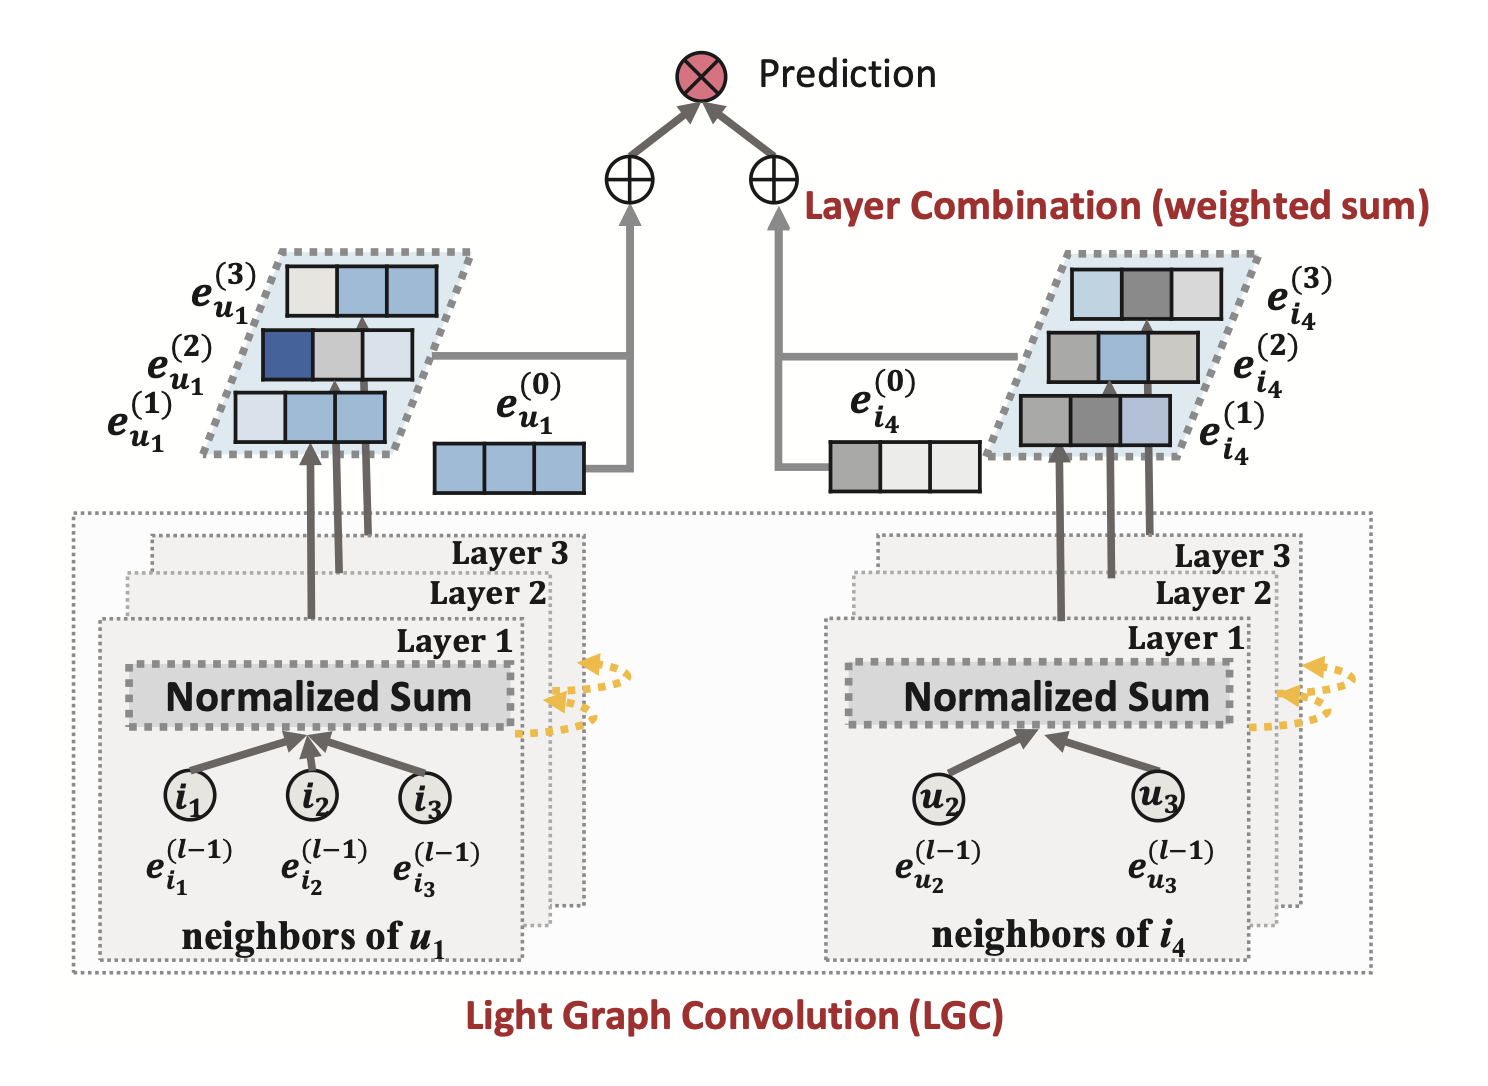
\includegraphics[scale=0.23]{assets/lgc_architecture.png}% 
    \figcaption{LGC Layer}% 
    \label{fig:impl:lgc_arch}% 
\end{minipage}

Between each layer, LightGCN uses the following propagation rule for user and
item embeddings.

\begin{equation}
    e_u^{(k+1)} = \sum_{i \in N_u} \frac{1}{\sqrt{|N_u|}\sqrt{|N_i|}}e_i^{(k)}
\end{equation}

\begin{equation}
    \quad e_i^{(k+1)} = \sum_{u \in N_i} \frac{1}{\sqrt{|N_i|}\sqrt{|N_u|}} e_u^{(k)}
\end{equation}

$N_u$: the set of all neighbors of user $u$ (items liked by $u$)

$N_i$: the set of all neighbors of item $i$ (users who liked $i$)

$e_u^{(k)}$ : k-th layer user embedding

$e_i^{(k)}$ : k-th layer item embedding

\subsection{Loss Function}

I have decided to use Bayesian Personalized Ranking (BPR)
loss~\cite{rendleBPRBayesianPersonalized2012}, as I think that pairwise
objective which encourages the predictions of positive samples to be higher
than negative samples for each user will properly reflect the given task.

\begin{equation}
    \begin{aligned}
        L_{BPR} & =                                                                                             \\
                & -\sum_{u = 1}^M \sum_{i \in N_u} \sum_{j \notin N_u} \ln{\sigma(\hat{y}_{ui} - \hat{y}_{uj})} \\
                & + \lambda ||E^{(0)}||^2                                                                       \\
    \end{aligned}
\end{equation}

$\hat{y}_{u}$: predicted score of a positive sample

$\hat{y}_{uj}$: predicted score of a negative sample

$\lambda$: hyperparameter which controls the L2 regularization strength